\documentclass{article}
\usepackage[utf8]{inputenc}

\title{Weak Lensing for Precision Cosmology}
\author{Mohamed Shaaban}
\date{April 2019}

\usepackage{natbib}
\usepackage{graphicx}
\usepackage{amsmath}
\usepackage{hyperref}
\begin{document}

\maketitle

\section{Introduction}
The most revolutionary discovery in cosmology since 
Hubble observed that the Universe is expanding is that 
this expansion is accelerating. A revelation that was 
awarded the 2011 Nobel Prize for its profound 
implications. \cite{nobel}. An accelerating
universe implies that either our understanding of gravity is flawed 
or that a mysterious pressure known as Dark Energy is driving the 
expansion \cite{peebles}.
This Dark Energy accounts for most (over 68\%) of the energy density in the observable universe, 
however its origin and physics are presently unknown \cite{planck}. 
As a result, the nature of Dark Energy is considered one of the 
greatest mysteries of modern science \cite{pathfinder}.  
\par
One of the most powerful techniques to probe Dark Energy and modified theories of gravity is weak lensing. Insert discription of weak lensing here \cite{hoekstra,rachel_2018}.
\par
Structure of the report

\section{Background Theory}
% \subsection{Notes}
% \begin{enumerate}
%     \item Motivate The Problem Cosmo
%     \item Introduce The Theory Cosmo + Lensing
%     \item Explain How Theory Solves The Problem
%     \item Current Results/ Experiments
%     \item Explain Problems with WeakLensing
%     \item Summarise
% \end{enumerate}

% Discuss probing the large scale universe with CMB, supernvae, clustering
% and lensing. 
% Note weak lensing makes no assumptions about the nature of dark matter
% and no assumptions about relationship between visible matter and mass therefore
% it provides a directly measured mass distribution in the universe as a function of 
% redshift. Therefore we can get info on DE and DM directly. It is sensitive to intial
% conditions so it can even give info on inflation. 
\subsection{Standard Model of Cosmology}
\begin{enumerate}
    \item Motivation (modified gravity vs Dark energy) is DE constant in space ? and time ?
    \item FRW Standard Cosmology 
    \item Distance Measures In Cosmo
    \item Gravitational Evolution of Dark matter
    \item Observables and Parameters
\end{enumerate}
The fundamental assumption in cosmology, known as the cosmological principle, is that we live in a homogenous and isotropic universe \cite{general_2013}. 
Remeber to show the Standard Model parameters! can be found in wikipedia.
\par Angular diameter distance is the one of relvance in lensing (distance measures in cosmology)
Distances in cosmo \cite{Hogg:1999ad}
lol 

\par For current and future surveys, one goal is to use the redshifts of the background galaxies (often approximated using photometric redshifts) to divide the survey into multiple redshift bins. The low-redshift bins will only be lensed by structures very near to us, while the high-redshift bins will be lensed by structures over a wide range of redshift. This technique, dubbed "cosmic tomography", makes it possible to map out the 3D distribution of mass. Because the third dimension involves not only distance but cosmic time, tomographic weak lensing is sensitive not only to the matter power spectrum today, but also to its evolution over the history of the universe, and the expansion history of the universe during that time. This is a much more valuable cosmological probe, and many proposed experiments to measure the properties of dark energy and dark matter have focused on weak lensing, such as the Dark Energy Survey, Pan-STARRS, and Large Synoptic Survey Telescope. 

\subsubsection{Matter Power Spectrum}
\cite{extragalactic}

\subsection{Bending of Light}
The fundamental concept on which weak lensing is built is gravity's ability to alter the path of a photon.
In this section we review the theory behind the bending of light necessary to develop the weak lensing formalism.
\subsubsection{Newtonian Lens}
\label{subsec:newtonlens}

It is a common misconception that the gravitational bending of light is an exclusive property of GR.
However, gravity induced alterations to a photon's path are predicted by newtonian mechanics \cite{lensingbook}. To illustrate this 
consider a mass $M$ located at the origin of the cartesian plane and a corpuscle(newtonian photon) 
propagating along the $x=b$ line (in this context $b$ is known as the impact parameter). 
Newton's second law predicts that the presence of the point mass will result in a momentum transfer
between the two objects. If the corpuscle starts with 
momentum $(p,0)$ then it will end up with momentum $(p_x,p_y)$.
Therefore, the particle path is deflected by some angle $\Delta \theta$. The deflection angle is 
simply given by 

\begin{equation}
  \sin(\Delta \theta) = \frac{p_y}{\sqrt{p_x^2+p_y^2}}
  \label{deflectionnewton}
\end{equation}


\par For very small deflections we have $p\approx p_x >> p_y$ and $\Delta \theta << 1$. 
Therefore \autoref{deflectionnewton} simplifies to $\Delta \theta
\approx \frac{p_y}{p_x}$. We now consider the infinitesimal deflection along the entire path of the photon with
$d\Delta \theta = \frac{dp_y}{p_x} = \frac{1}{px} dx \frac{dp_y}{dx}$. Therefore, we can find the deflection
angle by 

\begin{equation}
  \begin{split}
  \Delta \theta_N &= -\frac{1}{p_x} \int dx \frac{dp_y}{dx} \\
  &= -\frac{1}{cp_x} \int dx \frac{dp_y}{dt} = -\frac{1}{cp_x} \int F_y dx \\ 
  &= \frac{2GM}{c^2b}
  \end{split}  
  \label{newtonbend}
\end{equation}

We note that the mass of the corpuscle cancels out of the deflection equation. Therefore this equation applies
for massless particles i.e. photons. Therefore \autoref{newtonbend} provides a newtonian description for the 
bending of light \cite{lensingbook}.

\subsubsection{General Relativistic Bending of Light}
In this subsubsection I give a quick sketch of the bending of light in the context of general relativity,
for a more detailed calculation please consult \cite{GR1}.

\par The Einstein's field equations in the presence of a charge free static point mass is uniquely solved by 
the Schwarzchild metric \cite{GR1}. The Schwarzchild metric is

\begin{equation}
  ds^2 = \left ( 1-\frac{r_s}{r} \right )  dt^2 - \left( 1-\frac{r_s}{r}\right) ^{-1} dr^2 -r^2 d\Omega^2
  \label{schwarz}
\end{equation}

Where $r_s$ is the Shcwarzchild radius of the system given by $r_s=2 \mu = 2GM/c^2$. We can analyze the path of the photon from \autoref{subsec:newtonlens} by studying the geodesic equations of the metric and finding the conserved
quantities of the system. We can then combine the conservation equations with the tangent vector norm condition for a 
null path to get the shape equation of the system as 

\begin{equation}
  \frac{d\phi}{dr} = \frac{1}{r^2} \left(\frac{1}{b^2}- \frac{1}{r^2} \left(1-\frac{2\mu}{r}\right) \right)^{-1/2}
  \label{shapeeqbend}
\end{equation}

where $(r,\phi)$ are the photons position in 2D polar coordinates and $b$ is the impact parameter. Rewriting this equation
under the transformation of $r = 1/u$ and working pertrubatively around $u(\mu =0) = \frac{1}{b}\sin \phi
$ we get 

\begin{equation}
  u(\phi) \approx \frac{1}{b}\sin \phi + \frac{3\mu}{2b^2} \left(1+\frac{1}{3}\cos 2 \phi \right)
  \label{eq:pertshape}
\end{equation}

in the limit were $\phi << 1$ and $u \rightarrow 0$ \autoref{eq:pertshape} simplifies to $\phi = \Delta \theta_N =\frac{2GM}{c^2b} $. Geometrically the deflection is given by $\Delta \theta = 2\phi$ and therefore the deflection angle is

\begin{equation}
  \Delta \theta = 2\Delta \theta_N=\frac{4GM}{c^2b}
  \label{grbend}
\end{equation}

We conclude that general relativity predicts a factor of 2 greater deflection form a point mass than is predicted by newtonian mechanics. This relationship greatly simplifies the formalism developed for weak lensing. 

\subsection{Weak Lensing Formalism}
Now that we have a theoratical understanding of the Cosmological parameters we would like to measure as well as an understanding of how gravitational fields impact the path of light we are ready to develop the weak lensing formalism on which all weak lensing applications are built.
Talk about thin lens and how the formalism revloves around projecting newtonian potential onto the lens 2D surface.\cite{basicLens}

% Cosmology standard model and lensing formalism
% begin{enumerate}
%     \item Current observations imply w=-1 however that is no constraint on its evolution
%     \item The inital fluctation ins matter density produced by random quantum events therefore CLT tells us that is a gaussiam random field therefore power spectrum is enough to get all statistics
% \end{enumerate}


\section{Measuring Shear (Images to Catalogs)}
The weak lensing analysis process can be conceptually split into two parts; 1) converting images to catalogs of galaxy shapes and 2) extracting scientific results from shape catalogs. In this section we present a sample image to catalog pipeline. An overview of a weaklensing analysis pipeline is presented in \autoref{fig:pipe}.

\begin{figure}
    \begin{small}
        \begin{center}
            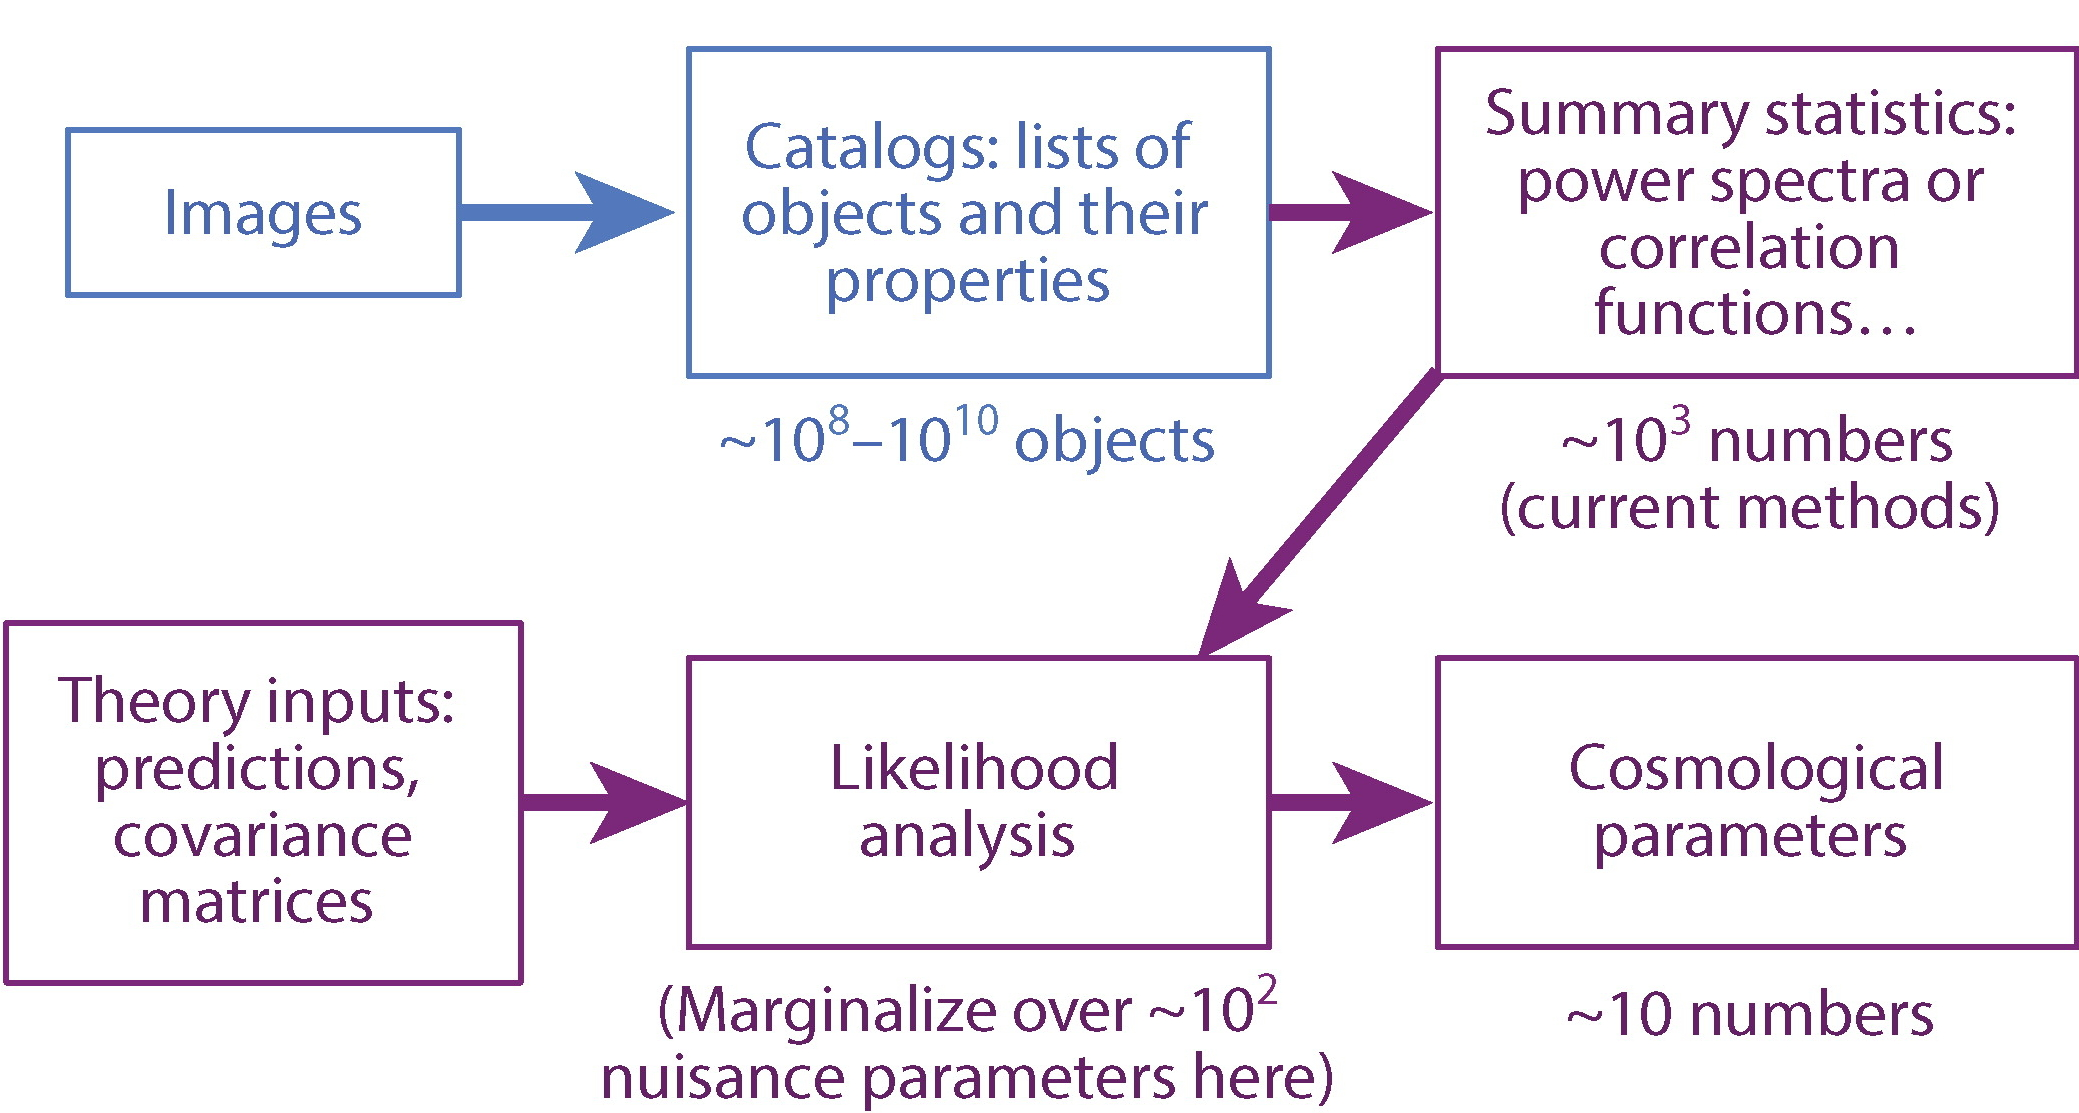
\includegraphics[width=0.95\textwidth]{figs/pipe.jpg}
        \end{center}
        \caption{A generic outline of weak lensing pipeline analysis as presented in \cite{rachel_2018}.}
        \label{fig:pipe}
    \end{small}
\end{figure}


\subsubsection{Object Detection}

The first step in weak lensing analysis is to detect the objects that will be analyzed. In the case of cosmological data the objects of interest are faint distant galaxies. Traditional methods for galaxy detection simply involve the detection of peaks above some detection threshold in a long exposure image. However due to the subtlety of the weak lensing signal the process is more involved. First we must confidently distinguish stars from galaxies, this is a fairly straight forward process that is usually done with photometric data. The next step is to detect galaxies that have blended together in the imaging process, i.e. detections with a double peak feature. Such blended images account for upto 10\% of detections and therefore need to be either deblended or discarded from the data set \cite{rachel_2018,general_2013}. Finally, based on the systematics of the detector some selection criteria is introduced that will filter out problematic images. 

\subsubsection{Shape Extraction}
After the galaxies are detected their shapes need to be measured. The accurate measurement of galaxy shape from an image is a rich and complex topic, we will state some results from \cite{massey_2013,general_2013} without derivation. Galaxy shapes can be quantified by computing the second moments of the galaxy images 

\begin{equation}
    Q_{ij} = \frac{\int  I(\vec{x}) W(\vec{x})x_ix_j d^2x}{}
    \label{eq:moments}
\end{equation}


The exact relationship between the the second moments and ellipticity is convention dependant, in this section we will use the same definitions as \cite{rachel_2018,Hoekstra:2013gua}. The complex ellipticity 

\begin{equation}
    R^2 = Q_{11} + Q_{22}
    \label{eq:size}
\end{equation}

\begin{equation}
    \epsilon = \frac{Q_{11}-Q_{22}+2iQ_{12}}{Q_{11}+Q_{22}}
    \label{eq:ellipticity}
\end{equation}

 

\subsubsection{Point Spread Function}

The point spread function (PSF) describes the response of an imaging system to a point source or point object. In practice the surface brightness profile of an object in an image is not the $I_{obs}$ from \autoref{eq:linearizedbright} but is convoloved with some unknown function $PSF(\vec{x})$. Therefore, in order to detect weak lensing signal we must understand and reconstruct our PSF in order to deconvolve it from the image. Deconvolving the PSF is the most important and most difficult step of any weak lensing analysis \cite{Hoekstra:2013gua,rachel_2018}. The PSF has a width which leads to rounder images and typically is anisotropic, which leads to a preferred orientation. The bias is grouped into two kinds: a multiplicative bias $m$ that scales the shear, and an additive bias $c$ that reflects preferred orientations that are introduced. The observed shear and true shear are thus related by

\begin{equation}
    \gamma_{obs} = (1+m) \gamma + c
     \label{eq:shearobs}
\end{equation}





\section{Catalogs to Science}
\subsection{Cosmic Shear}

\subsection{Cosmic Tomography}
For current and future surveys, one goal is to use the redshifts of the background galaxies (often approximated using photometric redshifts) to divide the survey into multiple redshift bins. The low-redshift bins will only be lensed by structures very near to us, while the high-redshift bins will be lensed by structures over a wide range of redshift. This technique, dubbed "cosmic tomography", makes it possible to map out the 3D distribution of mass. Because the third dimension involves not only distance but cosmic time, tomographic weak lensing is sensitive not only to the matter power spectrum today, but also to its evolution over the history of the universe, and the expansion history of the universe during that time. This is a much more valuable cosmological probe, and many proposed experiments to measure the properties of dark energy and dark matter have focused on weak lensing, such as the Dark Energy Survey, Pan-STARRS, and Large Synoptic Survey Telescope.
\cite{lensingbook} \cite{rachel_2018} \cite{hoekstra}


\section{Weak Lensing Results}
Some weak lensing results are already available from collocations such as DES and Subaru. These results include measurements of the power spectrum, contour constraint plots of $\Omega_m$ and $\sigma_8$, and tomogrophic data of the powers pectrum as a function of redshift. The results can be found in \cite{Subaru_2019}.

\section{Systematics}
Finally, we end this report with a discussion with a topic almost synonymous with weak lensing, systematic errors. Weak lensing has proven the most technically challenging cosmological probe due to the large range of systematic errors it suffers from \cite{general_2013}. Below We present a very brief overview over the rich topic of weak lensing systematics, for more details please see \cite{massey_2013,general_2013}.

\begin{enumerate}
    \item \textbf{PSF Errors:} As mentioned previously the PSF of the optical system needs to be estimated in order to extract meaningful data. This estimation involved interpolation between the systems response to a star, this interpolation is a less accurate representation of the PSF the further we get from a star. This uncertainty in the PSF could result in systematically introducing additional shear in a subset of the data and therefore detecting false signals. 
    \item \textbf{Blending:} As discussed previously approximately 10\% of the galaxies observed have some form of blending. This introduces the following problem; we can be over aggressive with our blended object identification which could result in non blended objects being flagged as blended and unnecessarily tampered with or conversely we could be too lenient with our detection allowing blended objects into our analysis. Both cases would introduce a systematic error into our data. Additionally, even if our detection algorithm is perfect our deblending algorithm might not be which would induce a systematic in 10\% of the data.
    \item \textbf{Selection Bias:} Depending on the optical system used to detect the galaxies an algorithm is needed to filter out unusable objects. The reason an object is unusable could stem from PSF uncertainty, blending, detector systematics or any other reason. Imperfections in such algorithms could result in an implicit shape dependance on the selection, such a dependance introduces/removes shear signal from the data.
    \item \textbf{Intrinsic Alignment:} Finally, throughout this entire the report the fundamental assumption as been that galaxy orientations are randomly distributed. This assumption is not entirely true, factors such as proximity to other galaxies, angular momentum during formation, and location relative to the center of mass of a cluster all impact the alignment of galaxies. A good example of this is the fact that galaxies near the center of a cluster tend to be oriented in a manner such that they point towards the center\cite{rachel_2018}.
\end{enumerate}

\bibliographystyle{plain}
\bibliography{refs}
\end{document}
